\documentclass{article}
\usepackage{smc2016}
\usepackage{times}
\usepackage{ifpdf}
\usepackage[english]{babel}
\usepackage{todonotes}
\usepackage{listings}
\usepackage{cite}
\usepackage{textcomp}
\usepackage{xspace}
\usepackage{float}
\usepackage{acronym}
%user defined variables
\def\papertitle{Rethinking the audio workstation: tree-based sequencing with i-score and the LibAudioStream}
\def\firstauthor{Jean-Micha\"el Celerier}
\def\secondauthor{Myriam Desainte-Catherine}
\def\thirdauthor{Jean-Michel Couturier}

% adds the automatic
% Saves a lot of ouptut space in PDF... after conversion with the distiller
% Delete if you cannot get PS fonts working on your system.

% pdf-tex settings: detect automatically if run by latex or pdflatex

\usepackage[pdftex,
  pdftitle={\papertitle},
  pdfauthor={\firstauthor, \secondauthor, \thirdauthor},
  bookmarksnumbered,
  pdfstartview=XYZ
]{hyperref}

\usepackage{graphicx}
\usepackage[figure,table]{hypcap}

%setup the hyperref package - make the links black without a surrounding frame
\hypersetup{
    colorlinks,%
    citecolor=black,%
    filecolor=black,%
    linkcolor=black,%
    urlcolor=black
}

\title{\papertitle}

\threeauthors
{\firstauthor} {LaBRI, Blue Yeti \\
	Univ. Bordeaux, LaBRI, UMR 5800, ~\\ F-33400 Talence, France. \\  Blue Yeti, F-17110 France. \\ jcelerie@labri.fr}
{\secondauthor} {LaBRI, CNRS \\ Univ. Bordeaux, LaBRI, UMR 5800, ~\\ F-33400 Talence, France. \\ CNRS, LaBRI, UMR 5800, ~\\F-33400 Talence, France. \\  INRIA, F-33400 Talence, France. \\ myriam@labri.fr}
{\thirdauthor} {Blue Yeti, F-17110 France. \\ jmc@blueyeti.fr}

\newcommand*{\LibAudioStream}{\textsc{LibAudioStream}\xspace}
\newcommand*{\iscore}{\textsc{i-score}\xspace}
\newcommand*{\maxmsp}{Cycling 74' \textsc{Max/MSP}\xspace}
\newcommand*{\puredata}{\textsc{PureData}\xspace}
\newcommand*{\csound}{\textsc{Csound}\xspace}
\newcommand*{\supercollider}{\textsc{SuperCollider}\xspace}
\newcommand*{\abletonlive}{Ableton \textsc{Live}\xspace}
\newcommand*{\bitwigstudio}{Bitwig \textsc{Studio}\xspace}
\newcommand*{\fasttracker}{\textsc{FastTracker}\xspace}
\newcommand*{\cubase}{Steinberg \textsc{Cubase}\xspace}
\newcommand*{\protools}{Avid \textsc{Pro Tools}\xspace}
\newcommand*{\logic}{Apple \textsc{Logic Pro}\xspace}
\newcommand*{\samplitude}{Magix \textsc{Samplitude}\xspace}
\newcommand*{\jamomaaudiograph}{Jamoma \textsc{AudioGraph}\xspace}
\newcommand*{\integraframework}{\textsc{Integra Framework}\xspace}
\newcommand*{\openmusic}{\textsc{OpenMusic}\xspace}
\newcommand*{\MUSIC}{\textsc{MUSIC}\xspace}
\newcommand*{\drile}{\textsc{Drile}\xspace}
\newcommand*{\jamon}{\textsc{JamOn}\xspace}
\newcommand*{\wwise}{AudioKinetic \textsc{Wwise}\xspace}
\newcommand*{\fmod}{\textsc{FMOD}\xspace}
\newcommand*{\faust}{\textsc{Faust}\xspace}
\newcommand*{\kyma}{\textsc{Kyma}\xspace}
\newcommand*{\audiomulch}{\textsc{Audiomulch}\xspace}

\acrodef{TC}{Time Constraint}
\newcommand*{\cantabileperformer}{Cantabile \textsc{Performer}\xspace}
\newcommand*{\timeconstraint}{\ac{TC}\xspace}
\newcommand*{\timeconstraints}{\acp{TC}\xspace}

\begin{document}
\capstartfalse
\maketitle
\capstarttrue

\begin{abstract}
The field of digital music authoring provides a wealth of creative environments in which music can be created and authored: patchers, programming languages, and multitrack sequencers.
By combining the \iscore interactive sequencer to the \LibAudioStream audio engine, a new music software able to represent and play rich interactive audio sequences is introduced.
We present new stream expressions compatible with the \LibAudioStream, and 
use them to create an interactive audio graph: hierarchical stream and send - return streams.
This allows to create branching and arbitrarily nested musical scores, in an OSC-centric environment.
Three examples of interactive musical scores are presented: the recreation of a traditional multi-track sequencer, an interactive musical score, and a temporal effect graph.
\end{abstract}

\section{Introduction}
Software audio sequencers are generally considered to be digital versions 
of the traditional tools that are used in a recording studio: tape recorders, 
mixing desks, effect racks, etc.

Most of the existing software follow this paradigm very closely, with 
concepts of tracks, buses, linear time, which are a skeuomorphic reinterpretation of the multi-track tape recorder~\cite{bell2015skeuomorphism}.
At the other side of the music creation spectrum, we find entirely interaction-oriented tools, 
such as \maxmsp, \puredata, \csound, or \supercollider. 
They allow to create musical works in programming-oriented environments.
In-between are tools with limited interaction capabilities but full-fledged audio sequencing support, 
such as \abletonlive, or \bitwigstudio.
The interaction lies in the triggering of loops and the ability to change the speed on the fly but is mostly separate from the "traditional" sequencer integrated in these software.

In this paper, we present a graphical and hierarchical approach to interactive audio sequencing.
We integrate the \LibAudioStream audio engine in the interactive control sequencer \iscore.
This forms an audio sequencing software that allows to author music in a time-line 
with the possibility to arbitrarily nest sounds and effects and trigger sounds interactively 
while keeping the logical coherency wanted by the composer. 
An extension is introduced to arrange audio effects in an interactive temporal graph.
For instance, instead of simply applying a chain of effects to an audio track, it is possible to apply temporal sequences of effects: an effect would be enabled for ten seconds, then, if an external condition becomes true, another effect would be applied until the musician chooses to stop it.

We will first present the existing works in advanced audio sequencing and workstations, 
and give a brief presentation of both \iscore and the \LibAudioStream.
Then, the new objects introduced in order to integrate these software together, allowing 
for rich audio routing capabilities, will be explained.
Finally, three examples of usage in the graphical interface of \iscore will be provided : a recreation of a standard multi-track player, an interactive score, and an effect graph applied to a sound.

\section{Existing works}
Outside of the traditional audio sequencer realm, there are
multiple occurences of graphical environments aiming to provide 
some level of interactivity.

M{\"o}llenkamp presents in~\cite{mollenkampparadigms} the 
commons paradigms for creating music on a computer: score-based with \MUSIC and \csound, 
patch-based with \maxmsp or \puredata, programming-based with \supercollider and many of the other music creation languages, music trackers such as \fasttracker which were used to make the music in old video game consoles, and multitrack-like such as \cubase, \protools.
\abletonlive and \bitwigstudio are given their own category thanks to the ability to compose clips of sound interactively.

\drile~\cite{berthaut2010drile} is a virtual reality music software. 
Loops are manipulated and bound together in a 3D environment. 
Hierarchy is achieved by representing the loops in a tree structure.

\kyma~\cite{scaletti1989kyma} is a hybrid software and hardware environment for sound composition. 
It offers multiple pre-made facilities for sound creation such as multi-dimensional preset interpolation, sound composition by addition and mutation, and sequential \& parallel sound composition on a time-line.

\audiomulch~\cite{bencina2005metasurface} is an environment for live music performance, which also provides preset space exploration thanks to the Metasurface concept. 
\cantabileperformer\footnote{\url{https://www.cantabilesoftware.com/}} is also an environment geared towards live performance, with the ability to trigger sounds, and a temporal ordering. It is closer to the cue metaphor than the sequencer metaphor.

Mobile and web applications are also a way that is more and more used to create music, 
but their are often embedded in a bigger score or framework and act more as an instrument than other systems.
An interesting example of web-based sequencer is \jamon~\cite{rosselet2013jam} which allows multiple persons to author music interactively in collaboration by drawing in a web page.
A deeper overview of the collaborative music authoring environments is given in~\cite{fencott2013computer}.

Finally, modern video game music engines such as \fmod and \wwise allow some level of interactivity: when some event occurs in a video game, then a sound will be played. 
Automation of parameters is possible, and these environments are geared towards three-dimensional positioning of sound and sound effects such as reverb, echo.

For low-level audio engines, one of the predominant methods is the audiograph.
Prime examples are \jamomaaudiograph~\cite{place2010jamoma} and \integraframework~\cite{bullock2011integra}.
Audio processing is thought of as a graph of audio nodes, where the output of a node can go to the input of one or multiple other nodes.
Audio workstations such as \samplitude (with the flexible plug-in routing) and \logic (with the Environment) provide access to the underlying audio graph.

\section{Context}
In this section, we will present the two tools that are used to achieve 
rich audio sequencing: \iscore and the \LibAudioStream.
\iscore is an interactive sequencer for parameters, which allows to position events 
in time, and gives the possibility to introduce interaction points and 
conditions in the score.
The detailed execution semantics are given in~\cite{celerier2015ossia}.

The \LibAudioStream~\cite{letzlibaudiostream} provides the ability to author audio expressions
by creating and combining streams. The notion of symbolic date, introduced in an extension of the library,
allows to start and stop the execution of streams at a date not known until the performance.

The goal of this work is to bind the audio capabilities of the \LibAudioStream 
with the \iscore execution engine and graphical interface, in order to allow 
the creation of rich hierarchic and interactive musical pieces.

\subsection{Presentation of i-score}
The original goal of \iscore is to communicate and orchestrate other software in a timely manner, 
through the OSC protocol.
The software can send automations, cue-like OSC messages at a given point in time, and call arbitrary JavaScript functions, in a sequenced environment.
It supports arbitrary nesting: a score can be embedded in another recursively.
This is similar to the notion of group tracks in many other sequencers, but without depth limit. 
Besides, there is no notion of "track" per se; rather, the composer works with 
temporal intervals which contains arbitrary data that can be provided by plug-ins.

Multiple possibilities of interactivity are provided in \iscore: trigger points, conditions, 
mappings, speed control.
\begin{itemize}
    \item Interactive triggers allow to block and synchronize the score until a specific event happens.
    For instance, when an OSC parameter fulfills a condition, such as  \lstinline[mathescape]!/a/b $\leq$ 3.14!, then 
    a part of the score can continue.
    \item Conditions allow to execute or disable part of the score according to a boolean condition.
    It makes if-then-else or switch-case programming constructs easy to implement in a temporal way.
    \item Mappings allow to map an input parameter to an output parameter, with a transfer function applied to the input.
    \item The execution speed of hierarchical elements can be controlled during the execution.
\end{itemize}

A span of time in \iscore might have a fixed or indefinite duration;
we refer to this span as a \timeconstraint since it imposes both a logical and temporal order to the elements before and after it.
 
A \timeconstraint may contain data by the form of processes: automations, mappings, but also loops and scenarios; a scenario is the process that allows nesting. 
When the \timeconstraint stops, all its processes are killed recursively.

\timeconstraints are linked together with Time Nodes, which allows for synchronization and branching of multiple streams of time.

An example of the temporal syntax of \iscore is presented in fig.~\ref{fig.iscore-example}.
It is for instance used by Arias and Dubnov in~\cite{Arias:VMO-Score} to construct a musical environment adapted to improvisation by segmenting pre-recorded audio phrases, to allow constrainted improvisation according to high-level musical structures.
The resulting generated structures bear similarity with the session concept in \abletonlive: one can loop dynamically over particular sections of a sound file. 

\begin{figure}
	\centering
	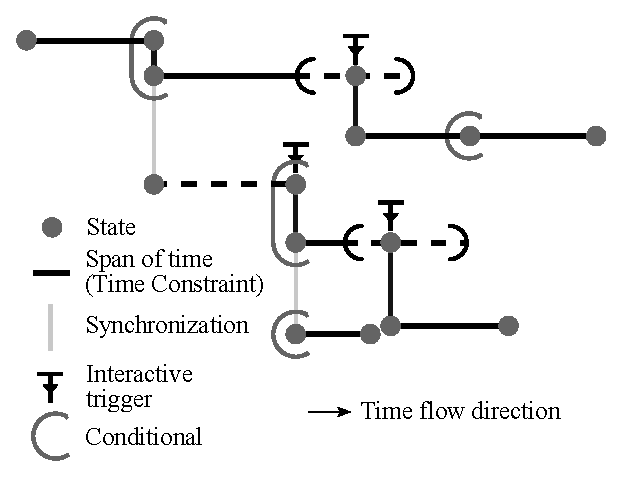
\includegraphics[width=0.45\textwidth]{figures/iscore-example.eps}
	\caption{Part of an \iscore scenario, showcasing the temporal syntax used. 
		A full horizontal line means that the time must not be interrupted, 
		while a dashed horizontal line means that the time of this Constraint can be interrupted to proceed 
		to the following parts of the score according to an external event.}
	\label{fig.iscore-example}
\end{figure}

\subsection{Presentation of the LibAudioStream}
The \LibAudioStream~\cite{letzlibaudiostream}, developed at GRAME, is a C++ library allowing to recreate the constructs commonly found in multi-track sequencers directly from code; it also handles communication with the soundcard hardware via the common audio APIs found on desktop operating systems.

One of the advantages of using a library instead of a graphical interface is that it provides scripting capabilities to the composer and makes algorithmic music composition easier.
It has been used with success in \openmusic~\cite{bouche2014programmation}.

Audio sounds and transformations are modeled by streams. 
An algebra with the expected operations is applied to these streams: serial and parallel composition, mixing, and multi-channel operations.
Streams are bound together in order to construct complex audio expressions.
For instance, two sound files can be mixed together with a Mix stream expression: 
\begin{lstlisting}[language=C++,columns=fullflexible,basicstyle=\ttfamily]
auto sound = MakeMixSound(
    MakeReadSound("a.wav"), 
    MakeReadSound("b.wav"), 
    0.75);
\end{lstlisting}
A stream can then be played through an audio player, with audio sample accuracy:
 
\begin{lstlisting}[language=C++,columns=fullflexible,basicstyle=\ttfamily]
StartSound(audioplayer, sound, date);
\end{lstlisting}

The play date must not necessarily be known in advance thanks to the notion of symbolic date.
Finally, \faust~\cite{orlarey2009faust} audio effects can be applied to the streams.

\section{Proposed audio system}
In this section, we will explain the audio routing 
features offered by the software.

First, we introduce new audio streams that allow a \LibAudioStream
expression to encapsulate the execution of a virtual audio player, 
in order to allow for hierarchy.

We make the choice to allow for hierarchy by mixing the played streams together.
This is done in accordance with the principle of least astonishment~\cite{seebach2001cranky} in mind for the composer: 
in most audio software, the notion of grouping implies that the grouped sounds will be mixed 
together and routed to a single audio bus.

Then, we present the concept of audio buses integrated to the \LibAudioStream,
with two special Send and Return streams.

Finally, we exhibit the translation of \iscore structures in \LibAudioStream expressions, 
which requires the creation of a dependency graph between audio nodes.

\subsection{Group audio stream}
In order to be able to apply hierarchical effects on the streams, 
and handle interactivity in recursive groups, we have to introduce a way to use sound hierarchy in the \LibAudioStream.

Our method employs two elements: 
\begin{itemize}
	\item A particular audio player that will be able to sequence the starting and stopping 
	of interactive sounds.
	Such players already exist in the \LibAudioStream but are tailored for direct output to
	the soundcard.
	\item A way to reintroduce the player into the stream system, so that it 
	is able to be pulled at regular intervals like it would be by a real soundcard while being mixed or modified by subsequent stream operators.
\end{itemize}

We introduce matching objects in the \LibAudioStream: 
\begin{itemize}
	\item A Group player. This is a player whose processing function has to be called manually. 
	Timekeeping supposes that it will be pulled in accordance at the clock rate
	and samplerate of the soundcard.
	\item A Group audiostream. This particular audiostream, of infinite length, 
	allows to introduce a Group player in a series of chained streams and takes care of having the Player process its buffers
    regularly.
    \item A finite loop audiostream.
    This stream loops over its content after a given duration.
\end{itemize}

The execution time of the hierarchized objects will be relative to the start time of the Group audiostream.

\subsection{Send and return audio streams}
In order to be able to create temporal effect graphs, we introduce another couple of objects.

The Send audiostream by itself is a passthrough: it just pulls the stream it is applied to.
It posseses the same definition: same length, same number of channels.
The Return audiostream, constructed with a Send stream, will make a copy of the data in 
the send stream and allow it to be used by the processing chain it is part of.
This means that a single sound source can be sent to two effect chains in parallel, for instance.

The Return stream is infinite in length: to allow for long-lasting audio effects 
like reverb queues or delays, we suppose that we can pull the data from the Send stream at any point in time.
If a Return stream tries to fetch the data of a Send stream that has not started yet, or that has already finished, a buffer of silence is provided instead.

The Send stream must itself be pulled regularly by being played as a sound, either directly or by a stream that would encapsulate it.

An example of such an audiostream graph is presented in fig.~\ref{fig.mixsendreturn}.

\begin{figure}[h]
	\centering
	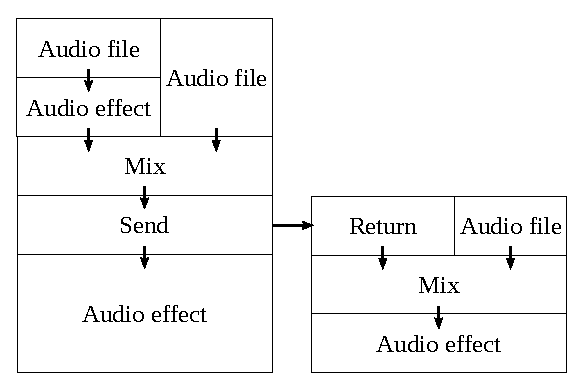
\includegraphics[width=0.45\textwidth]{figures/graph2.eps}
	\caption{An example of audio stream composition with the Send and Return objects. An arrow from A to B means that B pulls the audio data from A.}
	\label{fig.mixsendreturn}
\end{figure}

\subsection{Audio processes}
\label{sec.processes}
We provide multiple audio processes in \iscore, that map 
to the existing \LibAudioStream structures.

\begin{itemize}
	\item Effect chain process: register multiple audio effects one after the other. 
	For instance:~\\ \emph{Equalizer $\,\to\,$ Distortion $\,\to\,$ Reverb}. ~\\
	Currently only \faust effects or instruments are supported. 
    Interfaces are provided to allow the extension to other audio plug-in formats.
	\item Input process: allows to introduce the audio input of a sound card in the stream.
	\item Sound file: reads a sound file from the filesystem.
	\item Explicit send and return processes for manual routing.
	\item Mixing process: it exposes a matrix which allows to adjust the percentage of each sound-generating process going to each input process, send, and parent.
\end{itemize}

An important feature of audio workstations is the support for automation, that is, 
controlling the value of a parameter over time, generally with piecewise continuous functions.
In \iscore, automation is achieved by sending OSC messages to a remote software.
The OSC messages tree is modeled as an object tree.
We present the loaded effect plug-ins to this object tree, so that automations 
and mappings are able to control audio effects and audio routing volume.

A screen capture of a \timeconstraint with processes is given in fig.~\ref{fig.iscoreconstraint}.
\begin{figure}
	\centering
	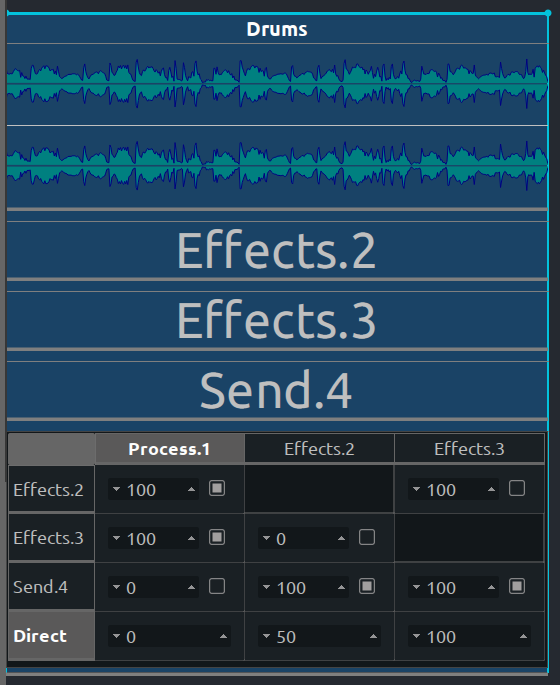
\includegraphics[width=0.35\textwidth]{figures/mix.png}
	\caption{An example of a \timeconstraint loaded with audio processes in \iscore. 
		Selecting a particular process shows a complete widget for editing the relevant parameters. On a single \timeconstraint, there can be only a single Mixing process (the table at the bottom), but there is no limit to the amount of other processes: there can be multiple sound files, etc.}
	\label{fig.iscoreconstraint}
\end{figure}

\subsection{Stream graph}
One problem caused by the presence of routing is that it is possible 
to create a data loop: if a Send is directly or indirectly fed its own data through a Return, 
the output would be garbage data: the Return would be asked to read 
the currently requested output from the Send which has not been written yet.

To prevent this, we create a graph where: 
\begin{itemize}
	\item Vertices are the sound generating elements associated to their output send: audio file reader, hierarchical elements, etc.
	\item Edges are the connections going from a send to a return, or from an element to the element it is mixed in.
\end{itemize} 

The graph, implemented with the Boost Graph Library~\cite{siek2001boost} can then be used to 
check for acyclicity. 
The user will be notified if that is not the case.
%As a byproduct of the imposed acyclicity of the graph, some level of parallel processing may be achieved, as long as causality is respected between nodes. 
%For instance, if two Returns with each their own effect chain are connected to a Send, it is possible to compute these returns on different threads after the current buffer of the Send has been processed.

We provide here the method to build the graph:

% \todo{Disambiguate the user-created sends and the sends required for the model}
%\paragraph{Vertice creation}
Vertices are created recursively from the \timeconstraints in \iscore: an \iscore document is entirely contained in a top-level \timeconstraint.

First, we iterate through all the processes of the given constraint.
If the process is hierarchical (Scenario, Loop), then we call the algorithm recursively on the process.

In the case of the Scenario, it means that we call recursively on all its Constraints.
In the case of the Loop, we call recursively on its loop pattern Constraint.
In both cases, we create a Group vertice to model the process. 
Edges are to be added from each stream in the hierarchical time-line, to the group stream.

If the process is a send or a return, we create a corresponding vertice.
Then, we create inner Sends for all the streams and a vertice for the Constraint itself.

Once all the vertices are created, the edges are added as mentioned before.

\begin{figure}
	\centering
	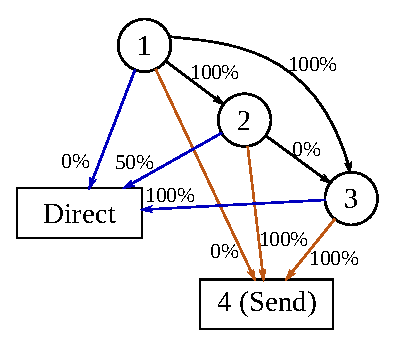
\includegraphics[width=0.35\textwidth]{figures/graph1.eps}
	\caption{Translation of the \timeconstraint of fig.~\ref{fig.iscoreconstraint} in a dependency graph.
		The edges in black represent the intra-Constraint connections. 
		The edges in blue (resp. orange) represent a connection to a visible output of 
		the Constraint. The percentages represent the level of mixing of the stream.
		\textit{Direct} corresponds to the signal that will be sent at the upper level of hierarchy.}
	\label{fig.graph}
\end{figure}

As mentioned before, there is an ordering between nodes of the graph: the parentmost vertice
has to be pulled before the others to reflect the causality.

%\todo{Comparer à Ableton ou il est possible pour chaque piste de choisir son entrée et sa sortie.}

Inside a \timeconstraint, causality also has to be enforced. 
Since a mixing matrix is provided, we have to ensure that an effect bus cannot be routed in 
itself in a loop. 
To prevent this at the user interface level, we disable by default the mixing of audio effect chains into each other. In fig.~\ref{fig.graph}, we show the resulting graph for a \timeconstraint. 

When the graph is verified acyclic, we perform the stream creation by iterating over the list of topologically sorted vertices.

%\todo{placement de la chaine de gain, time stretch, etc.}
\subsection{Stream creation}
We detail in this section the stream creation for particular elements.
\subsubsection{Scenario}
An \iscore scenario is an arrangement of temporal structures, as shown in fig.~\ref{fig.iscore-example}; it is a time-line of its own.
Since the execution and duration of these structures can change at run-time due to interactivity and hierarchy, it is not meaningful to directly use the tools provided by the \LibAudioStream: sequence stream, parallel stream, mix stream.
We instead use the Group player to organize our elements in time.

The creation of the Scenario stream is done as follows: 
\begin{enumerate}
	\item A Group player is created.
	\item For each Time Node in the scenario, a symbolic date is generated.
	\item For each \timeconstraint in the scenario, a stream is built; it is started and stopped at the symbolic date matching its start and end Time Nodes in the group player.
\end{enumerate}

The Audio stream of this process is the group player.
In order to enforce sample-accuracy whenever possible, if the i-score structures have a fixed date, we preset this date to its computed value.
If there is no interactivity involved, a sound following another will start at the audio sample one past the end of the first one. 
As soon as a sound's execution time is fixed, an algorithm checks for all the following sounds whose date could also be fixed.

\subsubsection{Loop}
Due to their interactive nature, loops in \iscore can be entirely different from 
one iteration to another. 
They are more similar to traditional programming language \texttt{do-while} constructs, than audio sequencer loops.
This prevents us from directly using the \LibAudioStream's loop stream, since it expects a looping sound of finite duration.
Instead, if the loop is interactive, we wrap the loop pattern \timeconstraint's audiostream in a Group player, reset the stream and start it again upon looping.
If the loop is not interactive, we can reset it at a fixed interval of time with the fixed loop stream introduced earlier.
This allows for sample accurate hierarchic looping with \iscore's processes semantics.

\subsubsection{Time Constraint}
As explained earlier, a \timeconstraint is a process container.
Such processes can be the sound processes presented in section~\ref{sec.processes}, and 
the control processes such as automation, etc.

The creation of the Constraint audio stream is done as follows: 
\begin{enumerate}
    \item For each sound-generating process, a stream and a send are created.
    \item For each effect chain, the effects are instantiated and an effect stream is created with a mix of the returns of the elements to which this effect applies.
    A send is also created.
    \item The mixing matrix is used to create mix audio streams from the sends and returns, which are routed either in the user-created sends, or in the stream corresponding to the \timeconstraint.
    A time-stretching audio stream is inserted before the send: it is linked to the execution speed of the \timeconstraint in \iscore which can vary interactively.
\end{enumerate} 

\subsubsection{A note on real-time performance}
Since a real-time audio input is provided, we ought to be able to 
use the system as a multi-effect, hence with the lowest possible latency.
The time-stretching effect itself may impose a latency high enough to make 
playing through the system impossible.

To solve this, when creating the graph, the parents of each Input node are recursively marked 
with a flag to indicate real-time processing. 
The \timeconstraints with this flag will not be able to be time-stretched, and will only 
be affected by the latency due to the effects manually introduced by the composer.

%Cas de la boucle avec un coup A, un coup B selon la condition ? 
%-> exécution d'un timenode doit reset le flux.

%Piste send / return: permet de maintenir les queues de reverb.

%\subsection{Routing, multi-channels, etc.}
%-> mettre maquettes track mix

\section{Examples}
We present in this part three examples of usage of the presented system.

\subsection{Recreation of a multi-track sequencer}
The first example, in fig.\ref{fig.score1}, is a recreation of the multitrack audio sequencer metaphor, with the primitives presented in this paper.
 
This score has three tracks, \textbf{Guitar}, \textbf{Bass}, and \textbf{Drums}, which are implemented with three \timeconstraints.
Each \timeconstraint has a Sound process and an Effect process; the Mixing process is hidden for clarity.
The bass track is a looping one-note sound. Automations are applied either at the "track" level, as for the drums, or at the "clip" level, as for the guitar \textbf{outro} clip. 
However, in the model there is no actual difference between track and clip, it is solely a particular organization of the score.
 
\begin{figure}[h]
    \centering
    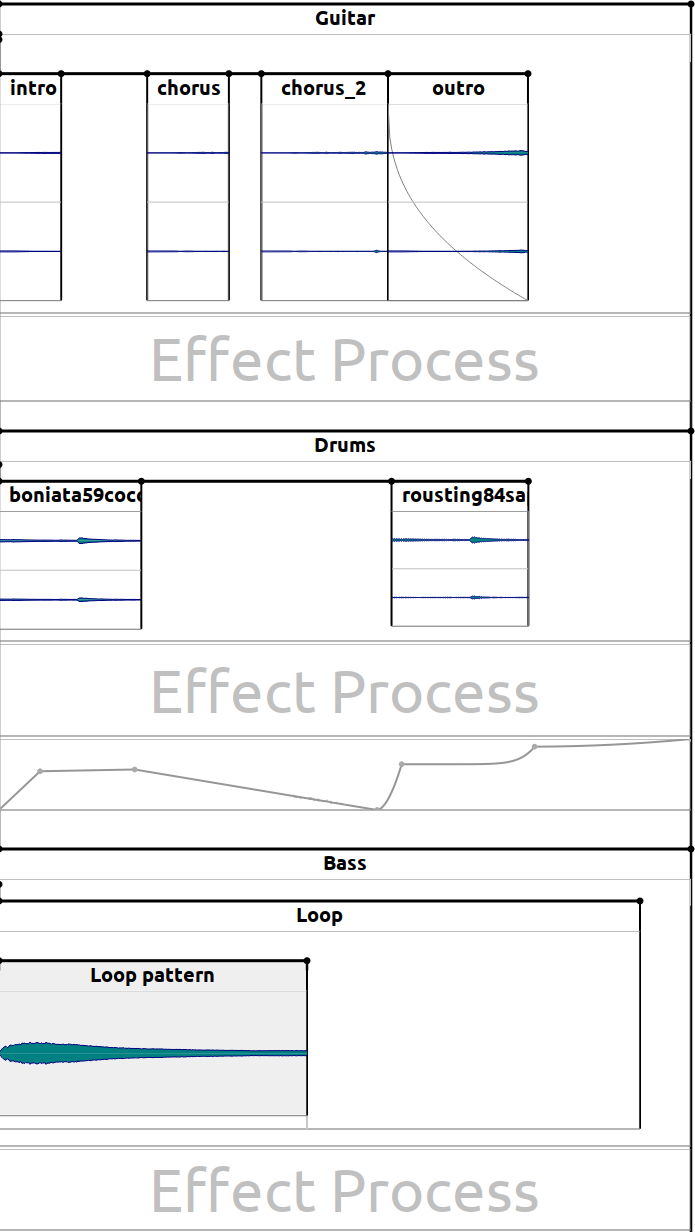
\includegraphics[width=0.45\textwidth]{figures/ex1.png}
    \caption{Multi-track sequencing.}
    \label{fig.score1}
\end{figure}

\subsection{Interactive scenario}
The second example, in fig.\ref{fig.score2}, gives an overview of the interactive possibilities when creating a song.

The score behaves as follows: 
For a few seconds, \textbf{intro} will play.  
Then, if an external event happens, like a footswitch being pressed, 
multiple things may happen: 
\begin{itemize}
    \item In all cases, the \textbf{eqcontrol} part will play, and automate a value of a global effect.
    \item If a first condition is true (\textbf{case1}), then \textbf{case1.B} will start playing immediately, and \textbf{case1.A} will start playing after a slight delay. If another external event happens, \textbf{case1.A} will stop playing immediately.
    \item If a second condition is true, at the same time, \textbf{case2} will start playing.
    \item After \textbf{eqcontrol} finishes, a hierarchical scenario \textbf{outro} is played, which contains two sounds and a parameter mapping.
\end{itemize}
If no external event happens, after some time, when reaching the end of the triggerable zone delimited by the dashed line, the triggering occurs anyways.

\begin{figure}[h]
    \centering
    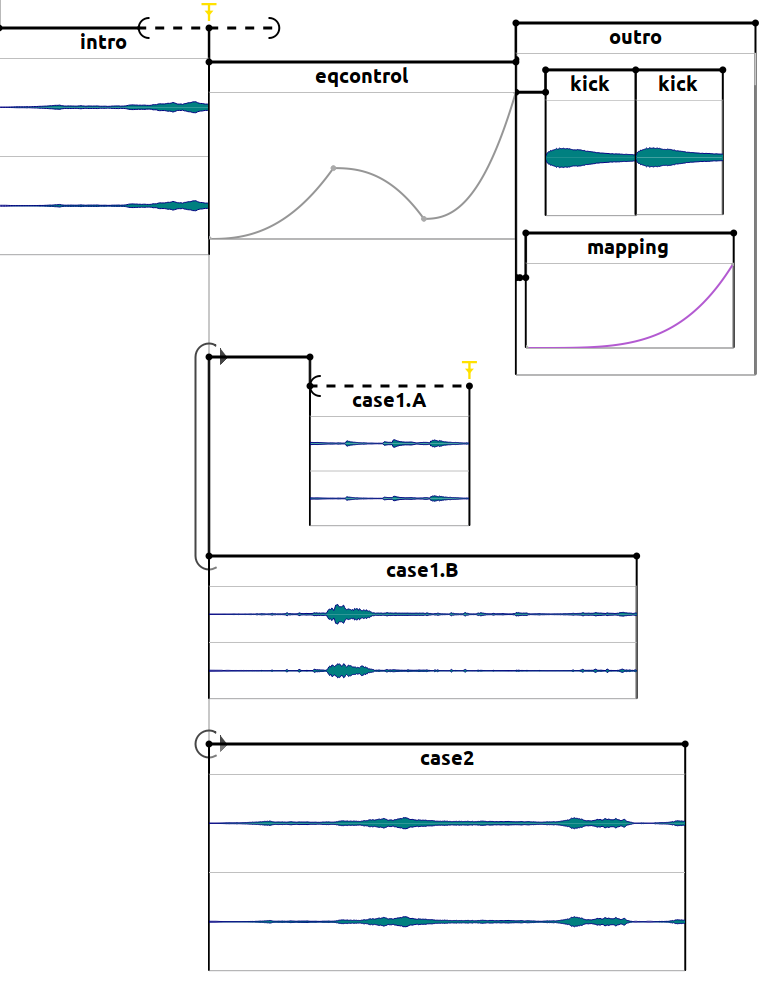
\includegraphics[width=0.45\textwidth]{figures/ex2.png}
    \caption{An interactive musical score.}
    \label{fig.score2}
\end{figure}
\newpage
\subsection{Temporal effect graph}
This last example, in fig.~\ref{fig.score3} shows how to arrange not sound, but sound processing temporally.
In this case, we have a sound playing, which is routed in the send process.
Then, a hierarchical scenario with multiple \timeconstraints is used. Two \timeconstraints have return processes connected to the previously created send.
Automations are applied to parameters of these effects.

\textbf{Second effect} will be triggered after an external event happens.
By using loops, effects, and \timeconstraints with infinite durations, this same mechanism would allow to simulate a guitar pedalboard with switchable effects, and the added possibility to create transitions between effects.

\begin{figure}[h]
    \centering
    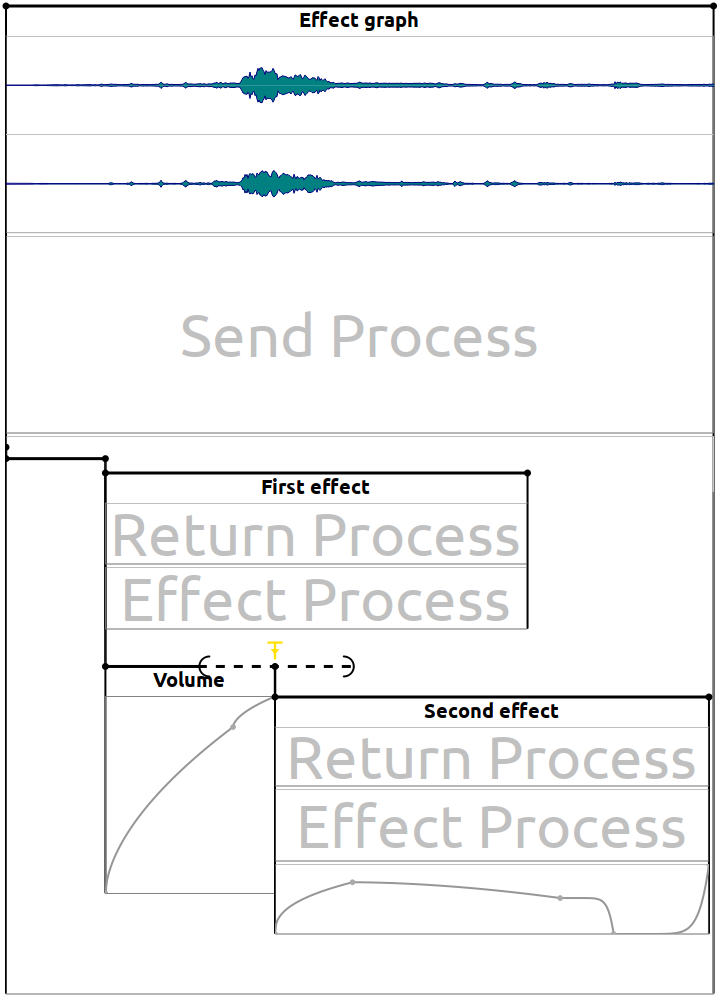
\includegraphics[width=0.45\textwidth]{figures/ex3.png}
    \caption{Temporal effect graph applied to a sound.}
    \label{fig.score3}
\end{figure}

\section{Conclusion}
We presented a computer system for creating interactive music, which extends the audio sequencer metaphor.
New kind of streams enabling hierarchy and audiograph-like behaviour are introduced to the \LibAudioStream, which is then binded to the \iscore primitives for specifying and scoring time and interaction.
Three examples present the various musical possibilities that are offered
through this system.

However, there are currently some differences with more traditional musical environments: for one, musical notation and concepts are absent from the system.
All the durations are expressed in seconds or milliseconds, instead of beats or any subdivision as they would in other environments. 
A possible extension to the \iscore execution engine would be to take into account beats for triggering, which would allow to synchronize multiple hierarchical loops to a beat and may be useful for some genres of music, such as electronica or rock.

Likewise, the system mostly handles audio and OSC data; MIDI is implemented at a primitive level.
Another unhandled question is effect delay compensation: sometimes, audio algorithms must introduce multiple frames of latency in their processing chain, for instance because they have to accumulate a certain amount of data.
This is not taken into account here, hence seemingly synchronized sounds may desynchronize themselves if this latency is not accounted for.

Finally, in many cases optimisations could be achieved to reduce the amount of data structures being created. For instance, when a single sound file is in a \timeconstraint, a simpler stream expression could be created.

The next steps for this research includes these points, work on sound spatialization, and interactive edition: modifying the score while it is already playing.

\begin{acknowledgments}
    This research was supported by the SCRIME (Studio de Création et de Recherche en Informatique et Musiques Expérimentales, \url{scrime.labri.fr}) which is funded by the French Culture Ministry. 
    SCRIME is a GIS (Group of interest in Science and Art) with University of Bordeaux, 
    Bordeaux INP, Bordeaux City, CNRS (National Scientific Research Center), Région Nouvelle Aquitaine (Aquitaine Regional Council) and the DRAC (Regional Direction of Culture).
	This work was also supported by an ANRT CIFRE convention with the company Blue Yeti under funding 1181-2014. 
\end{acknowledgments} 

\bibliography{smc2016template}

\end{document}
